% !TeX root = ../main.tex
% Add the above to each chapter to make compiling the PDF easier in some editors.

\chapter{Awareness}

This chapter reviews \gls{wa}, the structured, descriptive approach to the design of groupware. I will with introducing the \gls{sa}, one of the root concepts for the \gls{wa}.

\section{Situation Awareness}
% This section serves as a pre-cursor to the Workspace Awareness section, and shows the base that WA is built upon.

% TODO: state that situation awareness measures the awareness of the situation on all stages of information processing loop (perception=perception; comprehension=congition; projection=actions taken)

\gls{sa} originated in late 1980s and seen great development  due to its utility in jet fighter piloting simulations \parencite{endsley_situation_1988}. It is mostly used in attention-critical and hazardous tasks, where failure to react to the changes might lead to serious or even lethal consequences (i.e. operating a nuclear plant or a dam).
\parencite{endsley_design_1988} defines \gls{sa} as "the perception of the elements in the environment within a volume of time and space, the comprehension of their meaning, and the projection of their status in the near future". As such it is divided into 3 separate levels: perception, comprehension, and projection.

\parencite{endsley_situation_inbook} notes that the first step in gaining \gls{sa} is to "perceive the status, attributes, and dynamics of relevant elements in the environment". Going back to the jet fighter use case, the pilot has to keep track of all the different indicators in the cockpit. At the second level, more than the ability to take in all the need information is required, the pilot has to be able to comprehend the situation and highlight the important pieces of information with respect to the current goal. The difference between a novice and experienced pilot is that the former cannot achieve the second level of \gls{sa}, even if they were able to get the same information on the first level. Level 3 of situation awareness describes the ability of the user to employ their knowledge from the first and the second levels in order to predict the state of the system in the nearest future.

\paragraph{Measurement}
\parencite[p.~791-792]{endsley_situation_1988} reviews different approaches to the measurement of \gls{sa} that help system designers answer the fundamental question: "Does system A promote better SA than system B?". In her opinion, all the approaches that were available up to that point suffer from their own individual limitations. For example, the subjective approach, where the subject is asked to rate his \gls{sa} from 1 to 10 suffers from 2 major drawbacks: first, the subject is not aware of "what is really going on in the environment", and secondly, the outcome of the task can influence the rating. The psychological approach suffers from the incomplete human-computer interfaces to monitor what is going on with the user at this moment, and what they are thinking about. Finally, if the questionnaires are used, the fact that humans are not that good at recalling past mental events comes into play. Another set of problems arises, if an attempt is made to solve the issue with the questionnaire approach by querying users in real-time: they can start to attend to the information they are questioned upon more thoroughly, or they can be under a heavy attentional load at the moment, which would obstruct their answer.

Nevertheless, the biggest limitation of the mentioned approaches was that they attempted to evaluate only a single design issue at the time. This led \parencite{endsley_situation_1988} to the introduction of \gls{sagat} . First, the task goes though goal-directed analysis to determine the \gls{sa} requirements: the goal, subgoals, decisions required to actualize the given subgoal, and the knowledge required on all three levels of \gls{sa} (\ref{fig:sagoalorientedtaskanalysis}).
\begin{figure}
	\centering
	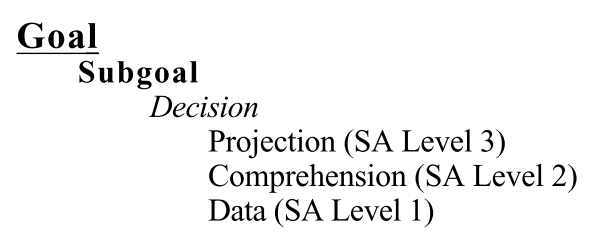
\includegraphics[width=0.7\linewidth]{figures/placeholders/SA_goal_oriented_task_analysis}
	\caption{Format of Goal-Directed Task Analysis. Source: \parencite{endsley_direct_nodate}}
	\label{fig:sagoalorientedtaskanalysis}
\end{figure}
This yields an extensive list of questions, which assess the \gls{sa} information of primary and secondary importance (example analysis can be seen the Table \ref{tab:sagoalorientedtaskanalysisresultexample}).
% Please add the following required packages to your document preamble:
% \usepackage{multirow}
\begin{table}[]
	\caption{Example of Goal-Directed Task Analysis for En-route Air Traffic Control. Adapted from: \parencite{endsley_direct_nodate}}
	\label{tab:sagoalorientedtaskanalysisresultexample}
	\begin{tabularx}{\linewidth}{X|l}
		\hline
		1.3 Maintain aircraft conformance                        & \textit{Subgoal}                            \\ \hline
		\hspace{.25cm}1.3.1 Assess aircraft conformance to assigned parameters & \textit{Decision}                           \\ \hline
		\hspace{.25cm}\hspace{.25cm}aircraft at/proceeding to assigned altitude?             & \multirow{2}{*}{\textit{L3: Projection}}    \\
		\hspace{.25cm}\hspace{.25cm}aircraft proceeding to assigned altitude fast enough?    &                                             \\ \hline
		\hspace{.25cm}\hspace{.25cm}\hspace{.25cm}time until aircraft reaches assigned altitude            & \multirow{3}{*}{\textit{L2: Comprehension}} \\
		\hspace{.25cm}\hspace{.25cm}\hspace{.25cm}amount of altitude deviation                             &                                             \\
		\hspace{.25cm}\hspace{.25cm}\hspace{.25cm}climb/descent                                            &                                             \\ \hline
		\hspace{.25cm}\hspace{.25cm}\hspace{.25cm}\hspace{.25cm}altitude (current)                                       & \multirow{3}{*}{\textit{L1: Perception}}    \\
		\hspace{.25cm}\hspace{.25cm}\hspace{.25cm}\hspace{.25cm}altitude (assigned)                                      &                                             \\
		\hspace{.25cm}\hspace{.25cm}\hspace{.25cm}\hspace{.25cm}altitude rate of change (ascending/descending)           &                                             \\ \hline
		\hspace{.25cm}\hspace{.25cm}aircraft at/proceeding to assigned airspeed?             & \textit{L3: Projection}                     \\ \hline
		\hspace{.25cm}...                                                      & \textit{}                                   \\ \hline
		1.3.2 Resolve non-conformance                            & \textit{Decision}                           \\ \hline
		\hspace{.25cm}...                                                      & \textit{}                                   \\ \hline
		...                                                      & \textit{}                                   \\ \hline
	\end{tabularx}
\end{table}
Next, the simulation is halted multiple times, and the pilots are queried on a randomly selected questions from the list. This is done to prevent giving away hints about current objective. When the simulation halts, all the control panels and other simulation elements are grayed-out. Not every pilot is queried on every question, the goal is to reach the desired statistical significance of the results by assessing a certain number of participants.

% This paragraph is a bit repetetive
By using \gls{sagat}, it is possible to get a snapshot of the current situation in the point of view of the pilot, which is unbiased by the recall difficulties, and that can be compared to the actual situation after the experiment. Additionally, pilots' \gls{sa} is not artificially enhanced, because the questions do not always directly address the main goals in the current situation, but can concern secondary information, which is still relevant.

\parencite{endsley_direct_nodate} notes that, since the introduction of \gls{sagat}, there is practical evidence that the method is valid, reliable, non-intrusive (in case of the halts are made at unpredictable time points), and is able to properly "reliably tap into memory stores" acting as a \gls{sa} index. 


\paragraph[Bridge]{}
Many ideas from the \gls{sa} concept are employed and adapted in the \gls{wa} framework.


\section{Workspace Awareness}
% Definition
\gls{wa} can be defined as "the up-to-the-moment understanding of another person’s interaction with the shared workspace" \parencite{gutwin_descriptive_2002}. While this is a trivial task in real-world, face-to-face collaboration, \gls{wa} becomes a bottleneck for productive collaboration because of the limited information that systems provide about their state changes, and their unfamiliar interaction interfaces.
 
% Description
It is an extension of the concept of \gls{sa}, research from the \gls{hci} and \gls{cscw} fields, as well as the authors' own observations and research \parencite{gutwin_descriptive_2002}. \gls{wa} can be characterized as an adaptation of \gls{sa} for the day-to-day working scenarios. This was desired, because: "sorting slides on a table does not seem very similar to air combat in a jet fighter" \parencite{gutwin_descriptive_2002}, or to architectural collaboration in immersive \gls{vr} environments. Another major difference between \gls{sa} and \gls{wa} is that besides maintaining their \gls{sa} and performing the domain (their personal) task, collaborators have to collaborate.

% Framework 'classification'
This leads \parencite{gutwin_descriptive_2002} to introduce the \gls{wa} framework, which provides a toolset for describing and analyzing medium-sized workspaces. The framework is applicable to real-time distributed groupware, and small mixed-focus collaboration groups busy with generation and execution tasks.
% Framework descriprion
The \gls{wa} framework is split in 3 parts:
\begin{description}
	\item[Part I] What information makes up \gls{wa}?
	\item[Part II] How is \gls{wa} information gathered?
	\item[Part III] How is \gls{wa} used in collaboration? 
\end{description}

In \textit{Part I} the authors address the information that collaborators might require from the workspace. While this can be any type of information, it can be categorized into the most common types. For example, the category "Who" deals with the presence, identity, and authorship questions, and contains the following questions: "Is anyone else in the workspace?", "Who is participating? Who is that?", and "Who is doing that?". An example for the "Who" category can be seen in Table \ref{tab:watechniquesforwhoquestions}. There are 8 categories of questions in the Part I of the framework: \textit{questions about the present} (\textit{Who?, What?, Where?}) and \textit{questions about the past} (\textit{How?, When?, Who? (past), Where? (past), What? (past)}). The \gls{wa} framework doesn't concern itself with the information about the future, because the authors consider this factor to be too not trivial and generally hard to account for in design, in general.
This part of the framework allows designers to compare and design awareness support in different groupware applications by providing a fixed vocabulary for describing their systems.

\textit{Part II} of the framework deals with the ways, in which the information can be delivered to the users. The authors review 3 ways, in which information can be communicated in the workspace: through \textit{bodies and consequential communication}, through \textit{artifacts and feedthrough}, and \textit{through conversation, gesture, and intentional communication}. While the name of latter speaks for itself, the former two deal with information transfer through the consequence of people's actions in the workspace, and the information emitted by the manipulated objects in the workspace (for example, a characteristic sound initiated by a person drawing in the workspace).
By considering the different ways in which the information transfer can occur, system designers can make an educated decision about what approach to use in a particular situation.

\textit{Part III} of the framework turns to the question of how we make use of the information we gather through \gls{wa}. Here we discover 5 types of activities that benefit \gls{wa} in some way: \textit{management of coupling}, \textit{simplification of communication}, \textit{coordination of actions}, \textit{anticipation}, and \textit{assistance} (see the summary in Table \ref{tab:summaryofactivitieswherwacanbeused}).
This part of the framework allows awareness designers consider different ways people make use of the awareness information, and decide where, whether, and how much of this information is required.

\begin{table}[]
	\caption{Workspace awareness techniques for “who” questions. Adapted from: \parencite{gutwin_descriptive_2002}}
	\label{tab:watechniquesforwhoquestions}
	\begin{tabularx}{\linewidth}{lX}
		\hline
		WA element (Who)            & Example interface techniques                                                                                                                                                                                                                                                                               \\ \hline
		Presence (Is anyone there?) & • Participant list. The most basic awareness display, the participant list shows who is currently logged in to the system (although several other types of awareness information can be added to this basic idea). Presence is shown by presence in the list.                                              \\
		& • Embodiment solutions (telepointers, view rectangles, avatars, video images). Since an embodiment is a representation of an actual person, presence is shown by the existence of the embodiment. In some cases, presence can also be heard if embodiments emit sound as they interact with the workspace. \\
		Identity (Who is that?)     & • Participant list identifies participants with a name or picture.                                                                                                                                                                                                                                         \\
		& • Embodiments show identity through visual characteristics of the representation, such as colour (telepointers or view rectangles), shape and appearance (avatars), or actual images (video techniques).                                                                                                   \\
		...                         & \\ \hline                                                                                                                                                                                                                                                                                                           
	\end{tabularx}
\end{table}


\begin{table}[]
	\caption{Summary of the activities in which workspace awareness is used. Source: \parencite{gutwin_descriptive_2002}}
	\label{tab:summaryofactivitieswherwacanbeused}
	
	\begin{tabularx}{\linewidth}{lX}
		\hline
		Activity                        & Benefit of workspace awareness                                                                                                                        \\ \hline
		Management of coupling          & Assists people in noticing and managing transitions between individual and shared work.                                                               \\
		Simplification of communication & Allows people to the use of the workspace and artifacts as conversational props, including mechanisms of deixis, demonstrations, and visual evidence. \\
		Coordination of action          & Assists people in planning and executing low-level workspace actions to mesh seamlessly with others.                                                  \\
		Anticipation                    & Allows people to predict others’ actions and activity at several time scales.                                                                         \\
		Assistance                      & Assists people in understanding the context where help is to be provided.                                                                             \\ \hline
	\end{tabularx}
\end{table}


The complete \gls{wa} framework is summarized in Fig. \ref{fig:waframework}.

\begin{figure}
	\centering
	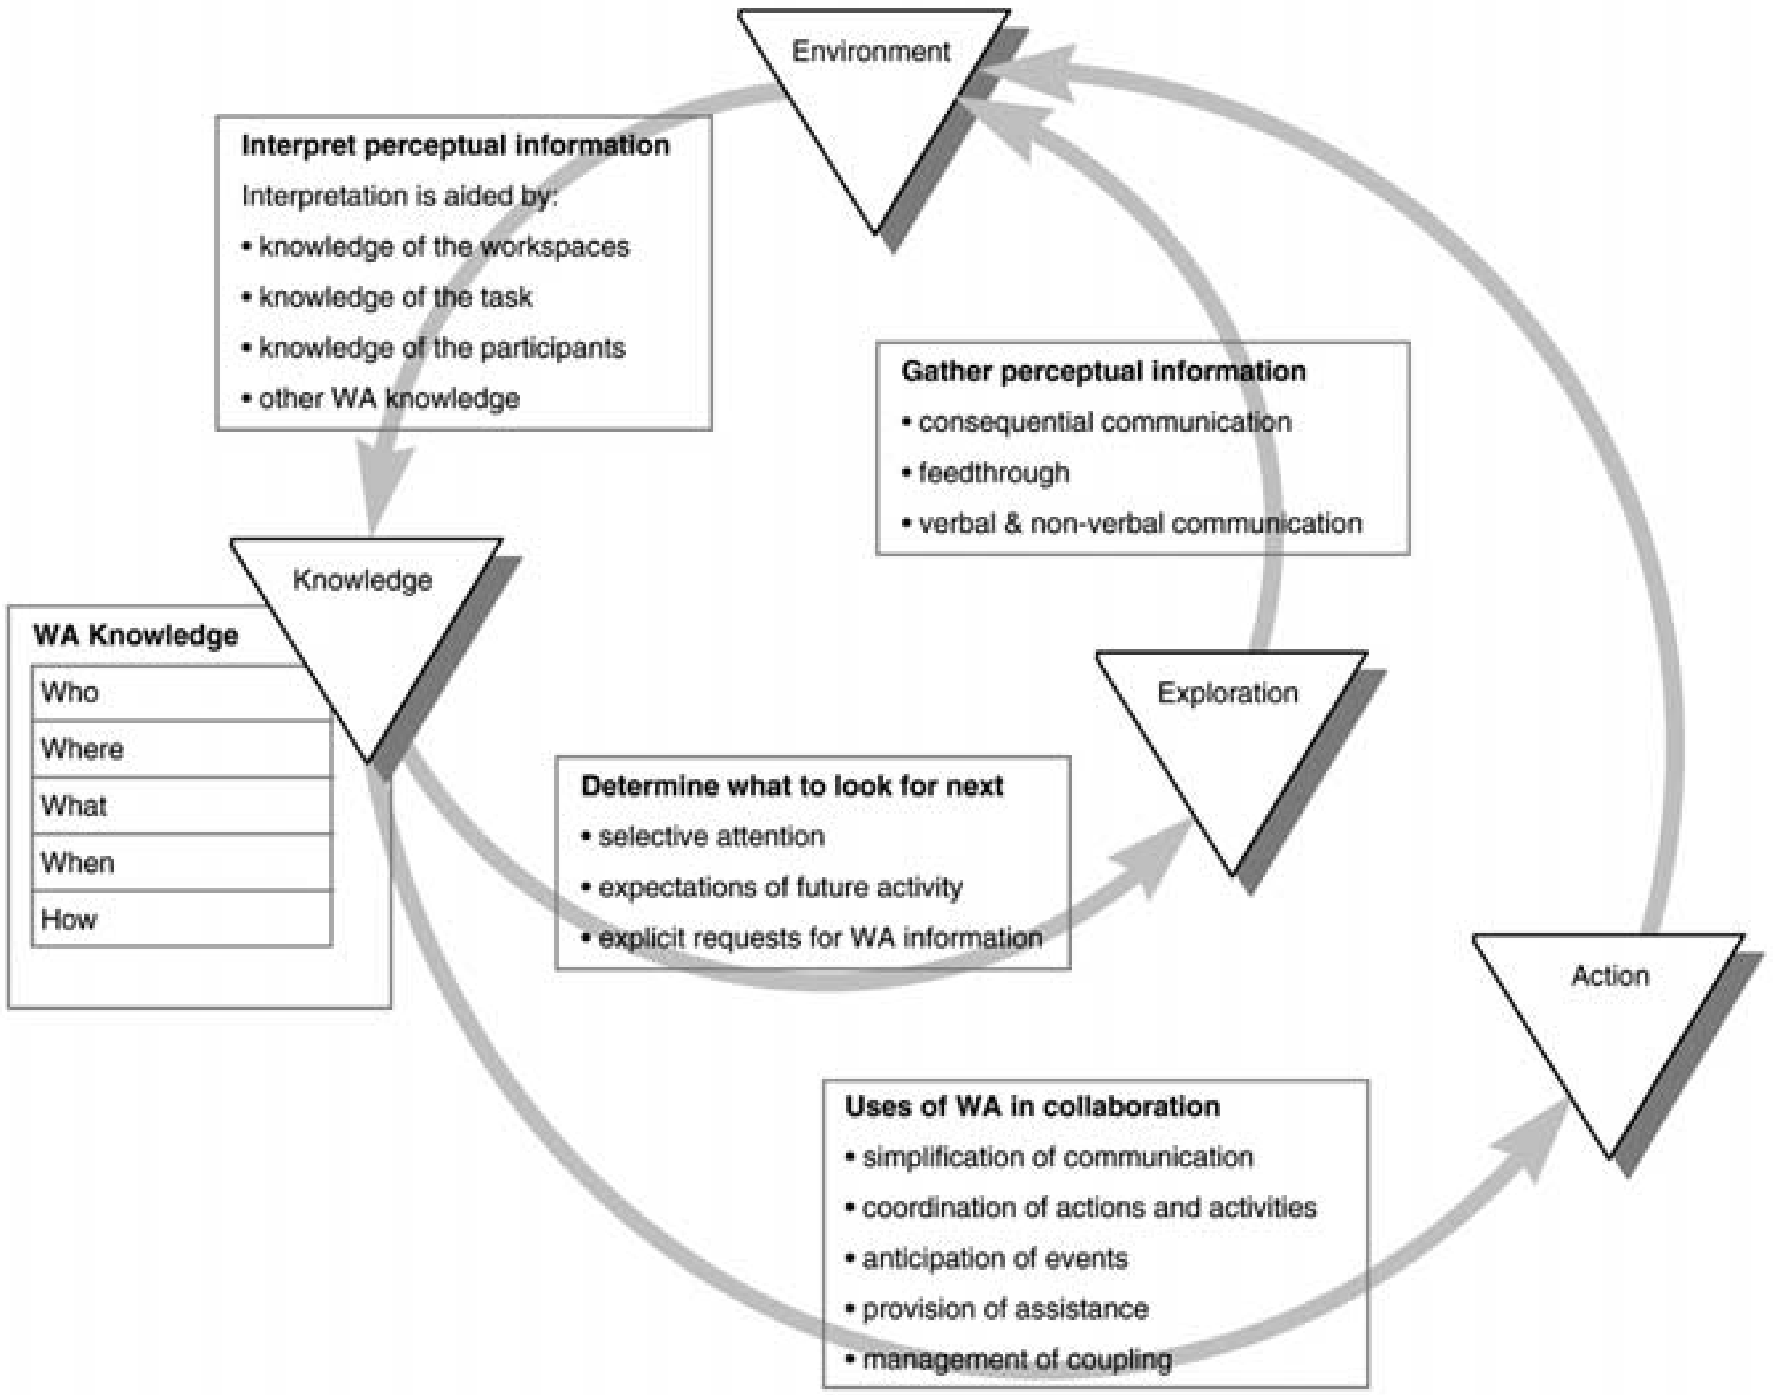
\includegraphics[width=0.7\linewidth]{figures/wa_framework}
	\caption{The \gls{wa} framework. Source: \parencite{gutwin_descriptive_2002}}
	\label{fig:waframework}
\end{figure}


\paragraph{Shared chalkboard application} 
\label{par:shared_chalkboard_application}
Gutwin et al. \parencite{gutwin_chalk_2011} employ the notion of \gls{wa} in their study about the effects of synthesized sound in a shared chalkboard \gls{cscw}.
%% What they explored, their focus and discoveries
%%% Goals
Two main goals of the study were to explore how much information can sound convey and the effectiveness of audio awareness in a \gls{cscw} application.

%%% Setup/system
The system was a 2D shared drawing application with one real (participant) and one simulated user (agent). The agent would draw multiple times in an off-screen part of the workspace at some point during the experiment. The participant had two tasks, primary and secondary. The primary task was to trace a given 2D shape (Fig. \ref{fig:gutwinchalk2011}), and the secondary was to keep track of what was happening in the shared workspace. When the participant and the agent drew, the system would emit a spatialized sound of chalk writing on a chalkboard. Participants had an additional way to monitor the shared environment -
%, or as authors call it - a type of awareness presentation,
the minimap (\textit{radar}), which showed the complete environment and the local chunk a participant was working in (indicated with a blue rectangle on the minimap, Fig. \ref{fig:gutwinchalk2011}).
% The workspace is seen in the figure
% Different awareness presentations - auditory and minimap
% Varying difficulty of the tracing shape

\begin{figure}
	\centering
	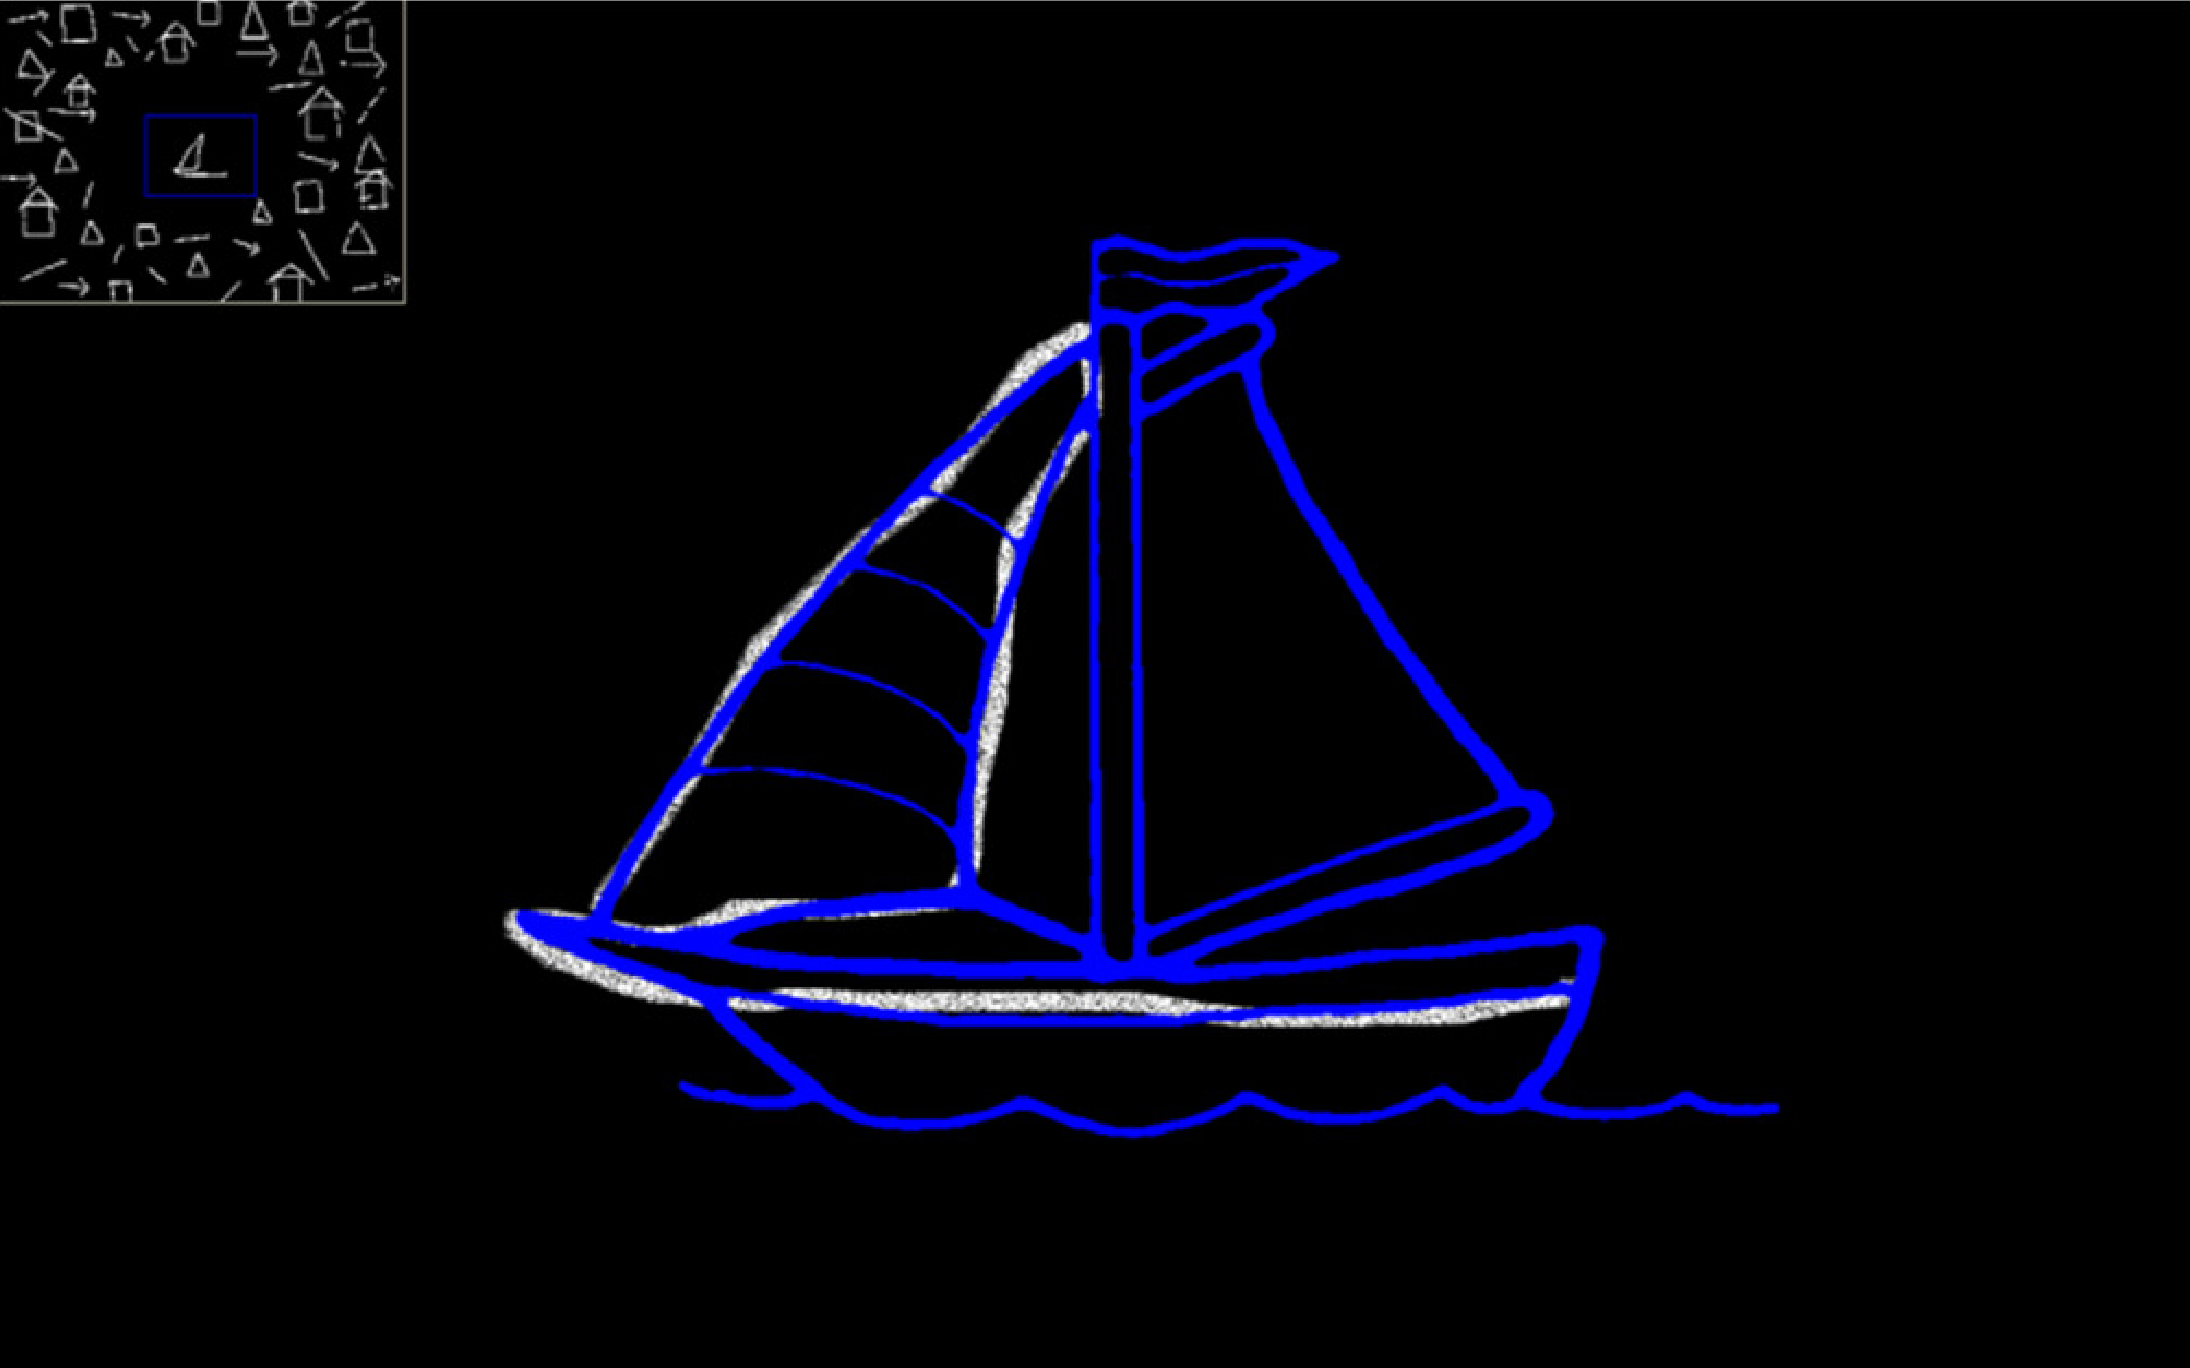
\includegraphics[width=0.7\linewidth]{figures/gutwin_chalk_2011}
	\caption{Shared chalkboard application, tracing shape and minimap. Source: \parencite{gutwin_chalk_2011}}
	\label{fig:gutwinchalk2011}
\end{figure}


%%% Focus and the results
\parencite{gutwin_chalk_2011} study one main independent variable: the type of awareness presentation. To keep most of the participants attention on the shape tracing task, one of the secondary independent variables was - attentional demand. It was implemented by making the tracing shape gradually move (0, 40, or 80 pixels/second movement), and thus requiring the participant to keep track of the shapes position. The other secondary independent variables were the workspace clutter and the size of the minimap.

The collected dependent measures were participants' accuracy in reporting \textit{what }type of figure the agent drew, \textit{where }and \textit{when }it drew it.
The authors used a \gls{sagat}-like approach for collecting the data: participants were tasked with pressing a space-bar as soon, as they noticed that the agent was drawing, and report aforementioned information.

The authors provide their thoughts regarding how and why the audio awareness helps in the collaborative scenarios, as well as the possible limitations of its application (i.e. sonifying actions with no obvious sound analogue, potential for distraction, and auditory clutter). They conclude significant improvements to the group awareness in cases, where it is hard to attend to the visual displays, or the line of sight is obscured.


\paragraph[Bridge to experiments]{}
One of the basic characteristics of awareness is that it is a secondary (monitoring) task - "the overall goal is not simply to maintain awareness but to complete some task in the environment" \parencite{gutwin_descriptive_2002}. This will be employed in the next chapter, in combination with the monitoring application of sonification, to study \gls{wa} in collaborative immersive \gls{vr} environment.